\chapter{Balanced Search Tree}
\section{2-3 Search Tree}
\subsection{Insertion}
Insertion into a 3-node at bottom:
\begin{enumerate}
\item Add new key to the 3-node to create a temporary 4-node.
\item Move middle key of the 4-node into the parent (including root's parent).
\item Split the modified 4-node.
\item Repeat recursively up the trees as necessary.
\end{enumerate}
\begin{figure}[hbtp]
\centering
\subfloat{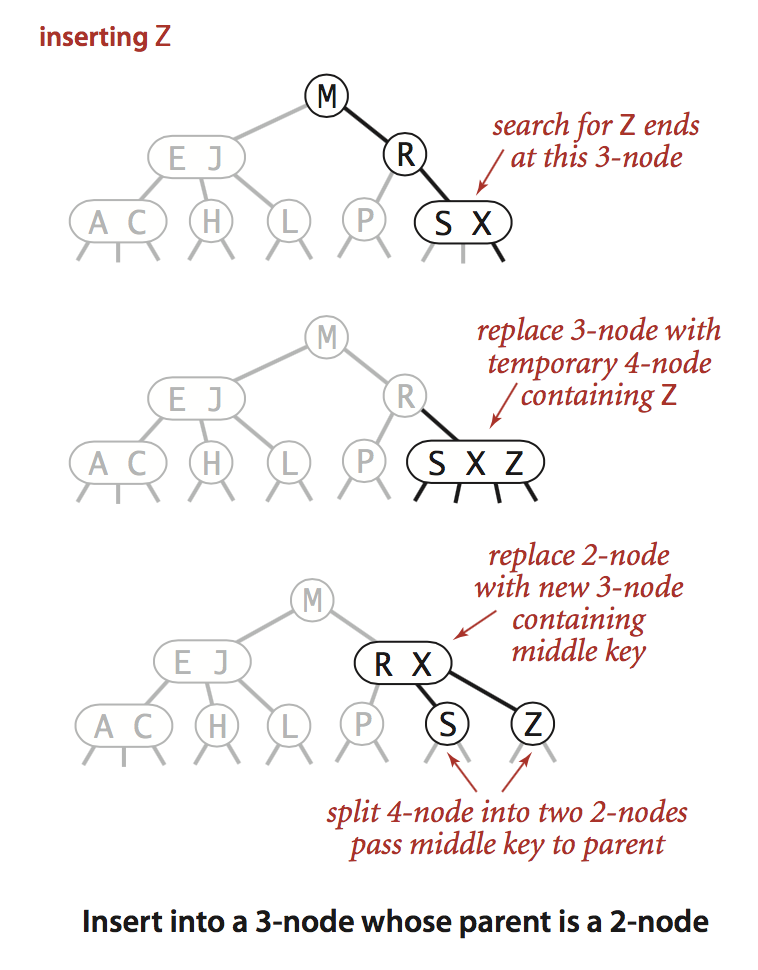
\includegraphics[scale=.8]{23insert1}}
\caption{Insertion 1}
\label{fig:LABEL}
\end{figure}

\begin{figure}[hbtp]
\centering
\subfloat{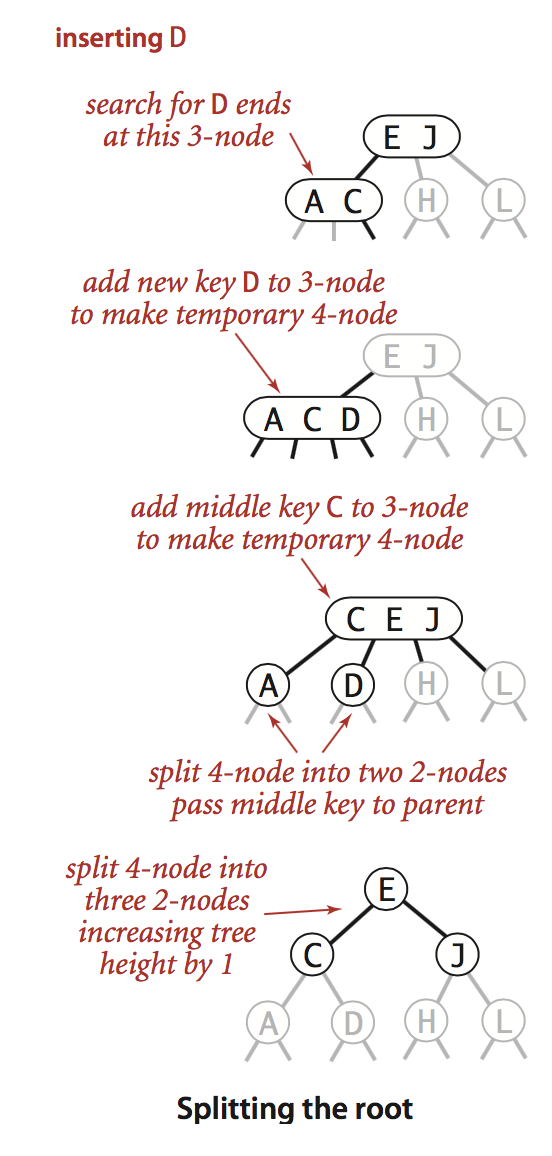
\includegraphics[scale=.8]{23insert2}}
\caption{insert 2}
\label{fig:LABEL}
\end{figure}

\subsection{Splitting}
Summary of splitting the tree. 
\begin{figure}[hbtp]
\centering
\subfloat{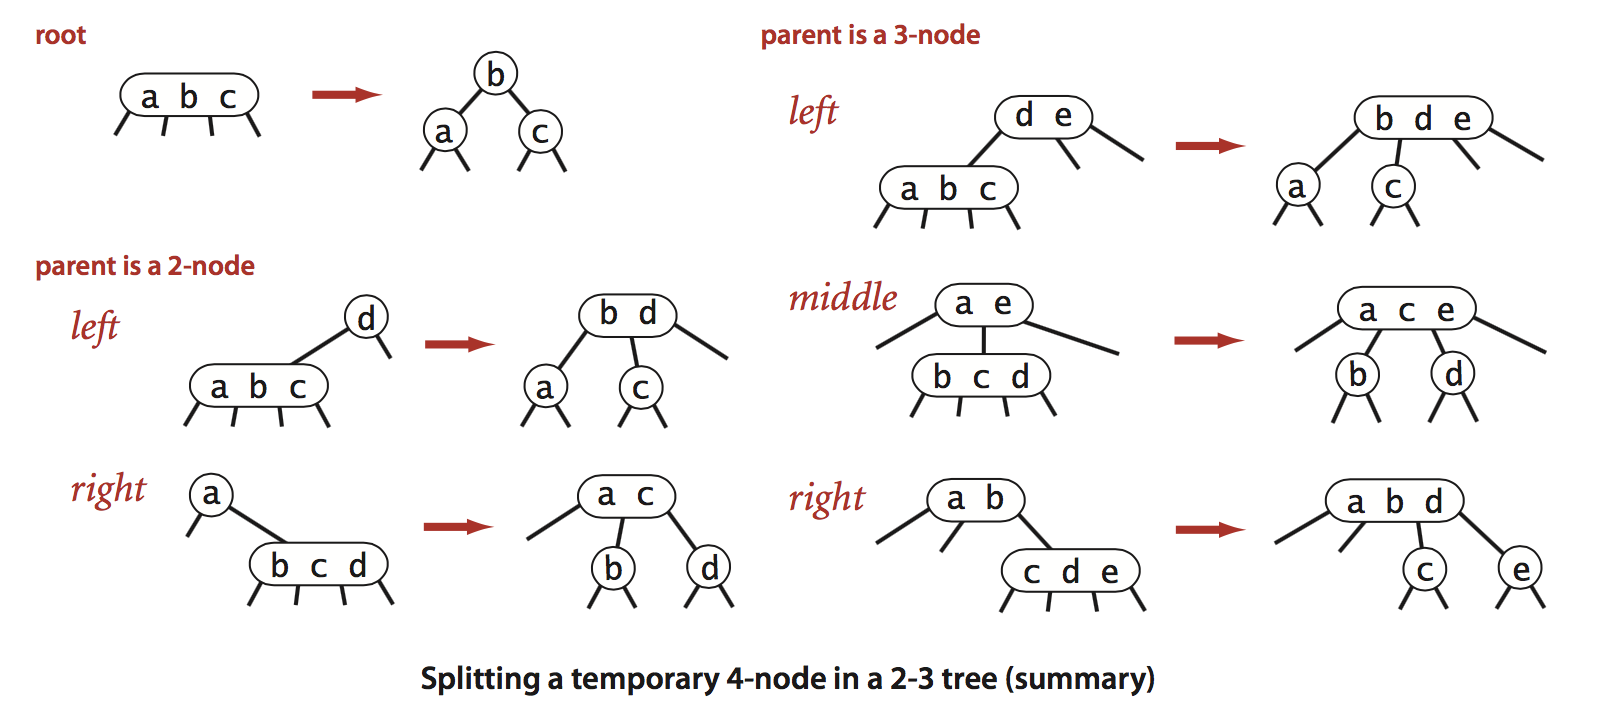
\includegraphics[scale=.65]{23splitting}}
\caption{Splitting temporary 4-ndoe summary}
\label{fig:splitting}
\end{figure}

\subsection{Properties}
When inserting a new key into a 2-3 tree, under which one of the following scenarios must the height of the 2-3 tree increase by one? When every node on the search path from the root is a 3-node

\section{Red-Black Tree}\label{rbtree}
\subsection{Properties}
Red-black tree is an implementation of 2-3 tree using \textbf{leaning-left red link}. \begin{figure}[hbtp]
\centering
\subfloat{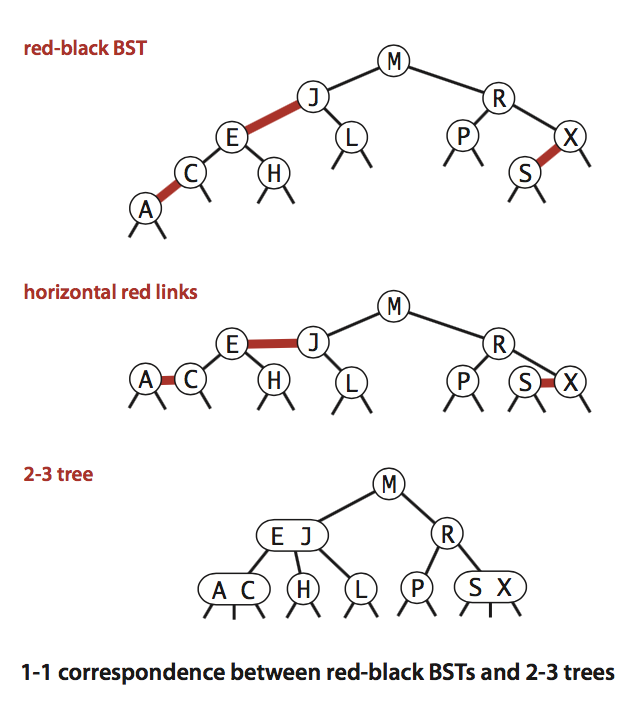
\includegraphics[scale=1.1]{rbtree11}}
\caption{RB-tree and 2-3 tree}
\label{fig:LABEL}
\end{figure}
The height of the RB-tree is at most $2\lg N$ where alternating red and black links. Red is the special link while black is the default link. 

\runinhead{Perfect black balance.}Every path from root to null link has the same number of black links.
\subsection{Operations}
\runinhead{Elementary operations:}
\begin{enumerate}
\item Left rotation: orient a (temporarily) right-leaning red link to lean left. Rotate leftward. 
\item Right rotation: orient a (temporarily) left-leaning red link to lean right. 
\item Color flip: Recolor to split a (temporary) 4-node. Rotate rightward. 
\end{enumerate}
\begin{figure}[hbtp]
\centering
\subfloat{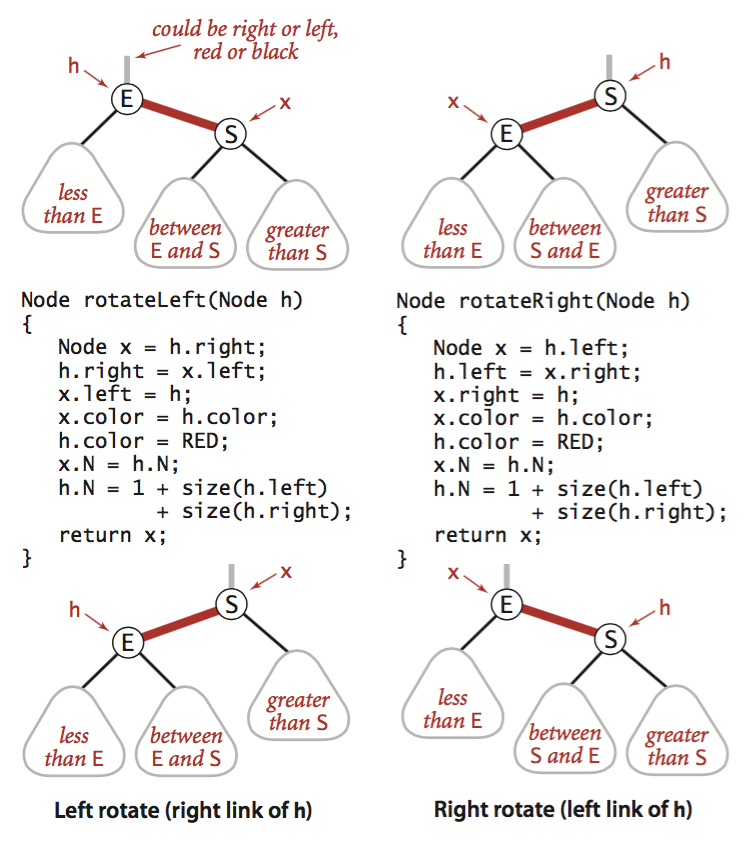
\includegraphics[scale=1.20]{rbrotate}}
\caption{Rotate left/right}
\label{fig:LABEL}
\end{figure}

\begin{figure}[hbtp]
\centering
\subfloat{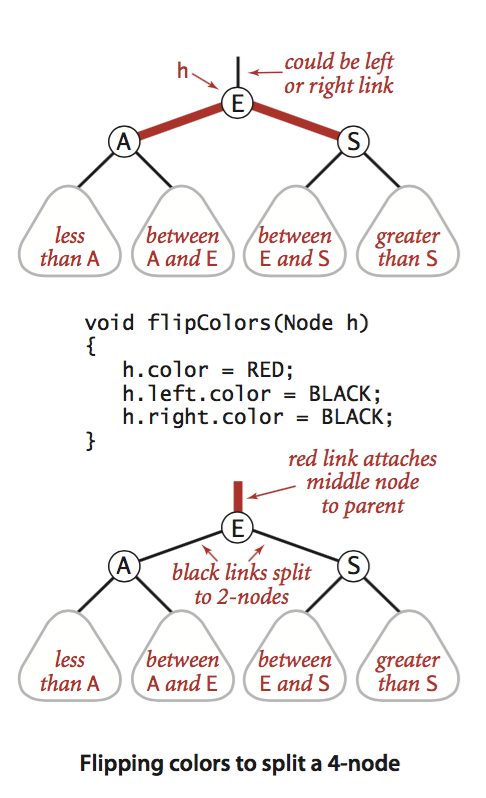
\includegraphics[scale=1.20]{rbflip}}
\caption{Flip colors}
\label{fig:LABEL}
\end{figure}

\runinhead{Insertion.} When doing insertion, from the child's perspective, need to have the information of current leaning direction and parent's color. Or from the parent's perspective - need to have the information of children's and grandchildren's color and directions.

For every new insertion, the node is always attached with red links. 

The following code is the simplest version of RB-tree insertion: 
\newpage
\begin{java}
Node put(Node h, Key key, Value val) {
  if (h == null)  // std red insert (link to parent).
    return new Node(key, val, 1, RED);
  int cmp = key.compareTo(h.key);
  if      (cmp < 0) h.left  = put(h.left,  key, val);
  else if (cmp > 0) h.right = put(h.right, key, val);
  else h.val = val; // pass

  if (isRed(h.right) && !isRed(h.left))    
    h = rotateLeft(h);
  if (isRed(h.left) && isRed(h.left.left)) 
    h = rotateRight(h);
  if (isRed(h.left) && isRed(h.right))     
    flipColors(h);

  h.N = 1+size(h.left)+size(h.right);
  return h; 
}
\end{java}

Rotate left, rotate right, then flip colors.

\runinhead{Illustration of cases.} Insert into a single 2-node: Figure-\ref{fig:rb_2}. Insert into a single 3-node: Figure-\ref{fig:rb_3}
\begin{figure}[t]
\begin{tabular}{cc}
  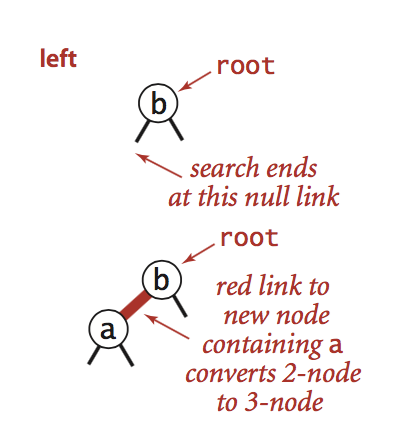
\includegraphics[height = 1.7in]{rb_left} &
  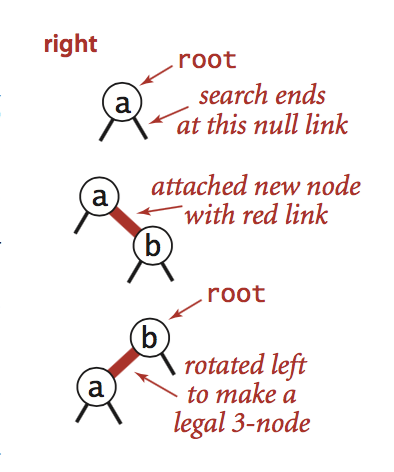
\includegraphics[height = 1.7in]{rb_right}\\
\end{tabular}
\caption{(a) smaller than 2-node (b) larger than 2-nod}
\label{fig:rb_2}
\end{figure}

\begin{figure}[t]
        \centerline{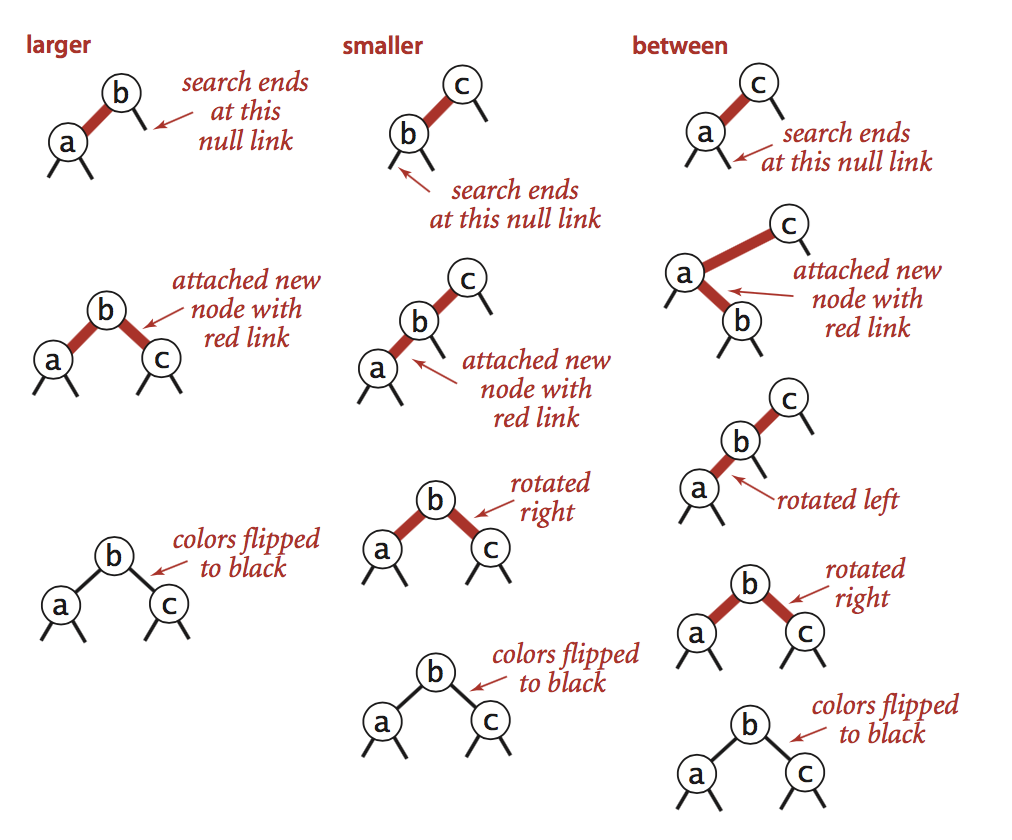
\includegraphics[height = 2.8in]{rb_3_left_right_btw}}
        \caption{(a) larger than 3-node (b) smaller than 3-node (c) between 3-node.}
    \label{fig:rb_3}
\end{figure}

\runinhead{Deletion.} Deletion is more complicated. 

\section{B-Tree}
B-tree is the generalization of 2-3 tree. 
\begin{figure}[hbtp]
\centering
\subfloat{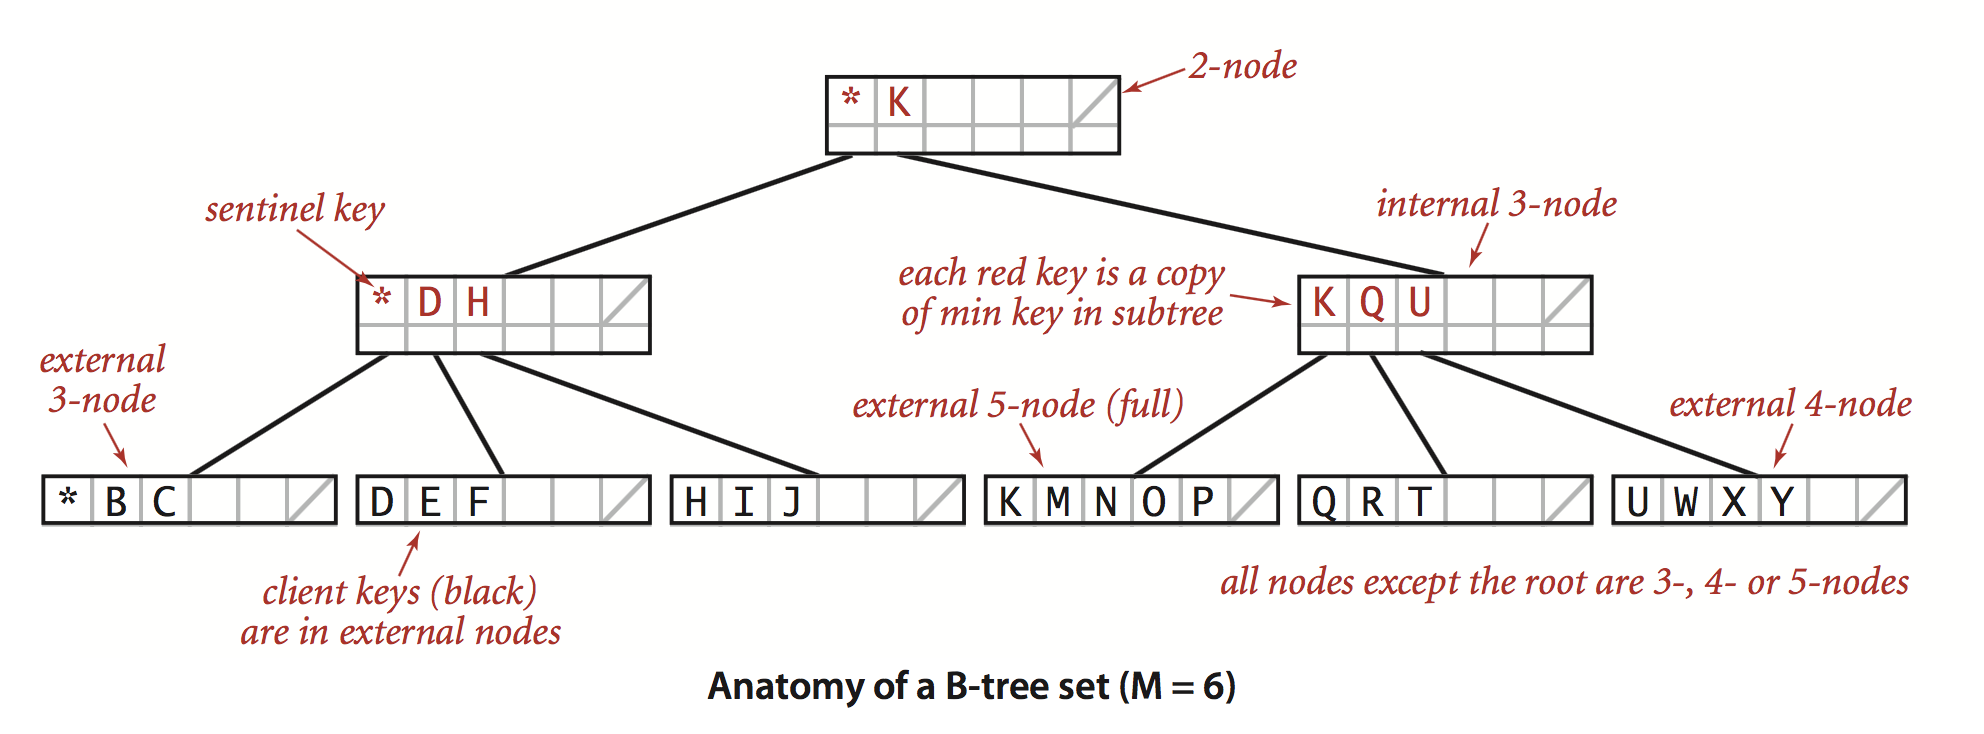
\includegraphics[scale=.50]{b-tree}}
\caption{B-Tree}
\label{fig:b-tree}
\end{figure}
\subsection{Basics}
Half-full principle: 

\begin{tabular}{lll}
\hline\noalign{\smallskip}
\textbf{Attrs} & \textbf{Non-leaf} & \textbf{Leaf} \\
\noalign{\smallskip}\hline\noalign{\smallskip}
Ptrs & \lceil\frac{n+1}{2}\rceil & \lfloor\frac{n+1}{2}\rfloor \\
\noalign{\smallskip}\hline\noalign{
\caption{Nodes at least half-full}
\end{tabular}

\subsection{Operations}
Core clues
\begin{enumerate}
\item \textbf{Invariant}: children balanced or left-leaning
\item \textbf{Split}: split half, thus invariant.
\item \textbf{Leaf-Up}: no delete, recursively move up the right node's first child;
thus invariant.
\item \textbf{Nonleaf-Up}: delete and recursively move up the left's last if left-leaning
or right's first if balanced; thus invariant. 
\end{enumerate}

\section{AVL Tree}
TODO

\section{Cartesian Tree}
\subsection{Basics}
Also known as max tree (or min tree). The root is the maximum number in the array. The left subtree and right subtree are the max trees of the subarray divided by the root number.
\begin{figure}[hbtp]
\centering
\subfloat{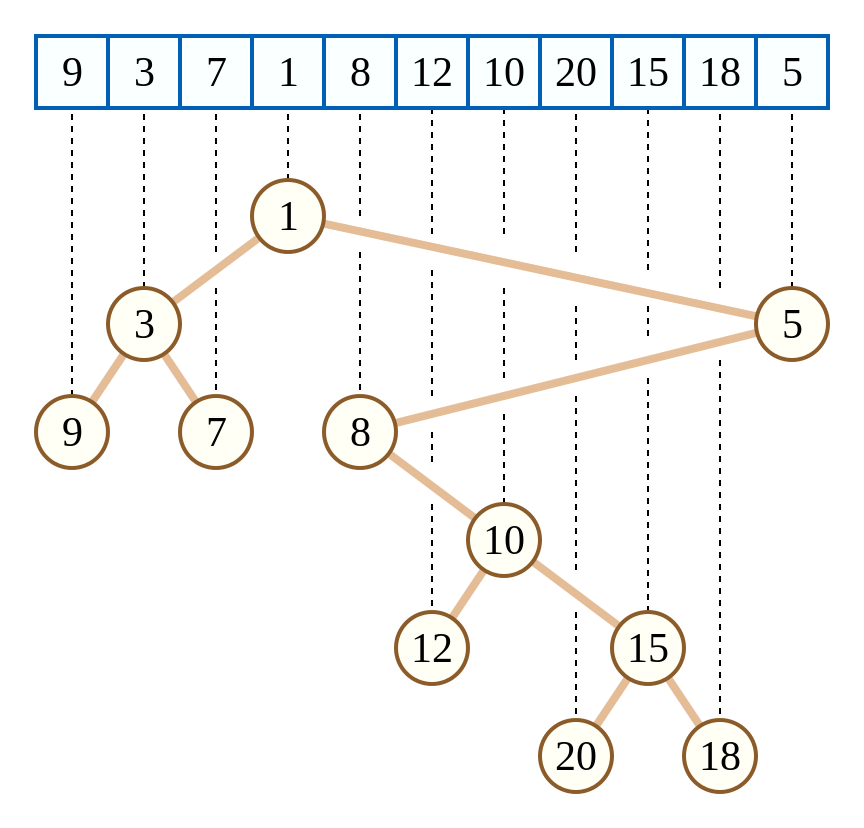
\includegraphics[scale=.60]{Cartesian_tree}}
\caption{Cartesian Tree}
\label{fig:cartesianTree}
\end{figure}
\begin{java}
Given [2, 5, 6, 0, 3, 1], the max tree is
     6
    / \
   5   3
  /   / \
 2   0   1
\end{java}
\runinhead{Construction algorithm.} Similar to all nearest smaller (or larger) values problem - Section \ref{allNearestSmaller}.

Core clues:
\begin{enumerate}
\item Use stack to maintain a \textit{strictly decreasing} stack, similar to find the all nearest large elements.
\itm Maintain the tree for currently scanning $A_i$ with the subarray $A[:i]$.
\begin{enumerate}
\item \rih{Left tree.} For each currently scanning node $A_i$, if ${stk}_{-1} \leq A_i$, then ${stk}_{-1}$ is the left subtree of $A_i$. Then pop the stack and iteratively look at ${stk}_{-1}$ again (previously ${stk}_{-2}$). Notice that the original left subtree of $A_i$ should become the right subtree of ${stk}_{-1} $, because the original left subtree appears later and satisfies the decreasing relationship.
\item \rih{Right tree.} In this stack, ${stk}_{-1} < {stk}_{-2}$ and ${stk}_{-1}$ appears later than ${stk}_{-2}$; thus ${stk}_{-1}$ is the right subtree of ${stk}_{-2}$. The strictly decreasing relationship of stack will be processed when popping the stack. 
\end{enumerate}
\end{enumerate}

$O(n)$ since each node on the tree is pushed and popped out from stack once.

\newpage
\begin{python}
def maxTree(self, A):
    stk = []
    for a in A:
        cur = TreeNode(a)
        while stk and stk[-1].val <= cur.val:
            pre = stk.pop()
            pre.right = cur.left
            cur.left = pre

        stk.append(cur)

    pre = None
    while stk:
        cur = stk.pop()
        cur.right = pre
        pre = cur

    return pre
\end{python}

Usually, min tree is more common. 
\subsection{Treap}
\rih{Randomized Cartesian tree}. Heap-like tree. It is a Cartesian tree in which each key is given a (randomly chosen) numeric priority. As with any binary search tree, the inorder traversal order of the nodes is the same as the sorted order of the keys.

\begin{figure}[hbtp]
\centering
\subfloat{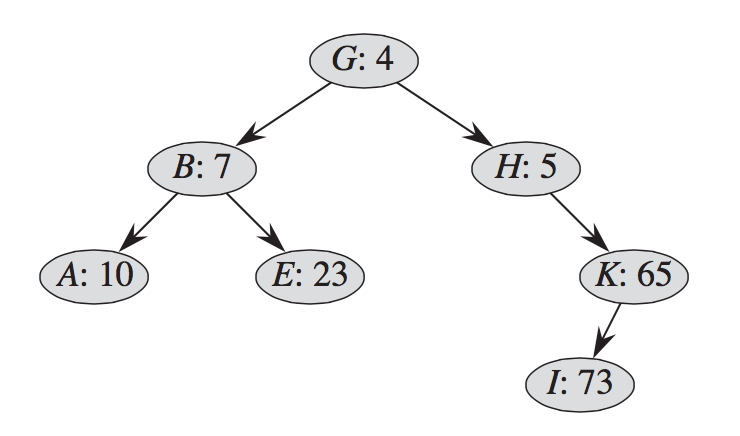
\includegraphics[scale=.80]{treap}}
\caption{Treap. Each node x is labeled with x.key: x.priority.}
\label{fig:treap}
\end{figure}

Construct a Treap for an array $A$ with index as the $x.key$ randomly chosen priority $x.priority$ $O(n)$. Thus support search, insert, delete into array (i.e. Treap) $O(\log n)$ on average. 

Insertion and deletion - need to perform \textit{rotations} to maintain the min-treap property. 
